\documentclass{article}
\usepackage{graphicx}

\title{Progress on the evaluation of ANLTR as a basis for FHiCL parsing}
\author{Mikhail Shiltsev}
\date{3rd of August, 2018}

	\addtolength{\oddsidemargin}{-.875in}
	\addtolength{\evensidemargin}{-.875in}
	\addtolength{\textwidth}{1.75in}

	\addtolength{\topmargin}{-.875in}
	\addtolength{\textheight}{1.75in}

\begin{document}

\section{Terminology}
    ANLTR

    	\quad ANTLR4, refering to the C++ runtime unless otherwise stated.\\ \\
    intermediate table 

    	\quad The intermediate data structure containing the configuration and extra debug information. Known as the paramset in my test code. \\ \\
    extendedval

    	\quad A container that has the value data from the document as well as additional information about the value. The exact structure is explained in section 5.2.  \\

    Each entry in the fhicl document will be an entry in the paramater set with the ID being the key and an extendedval as a value


\section{Where we are}

Functionality of current grammar
      
\quad The current version of the FHiCL grammar can recognize all key words stated in the quickstart guide and the FHiCL standard document. It also contains all parser rules required for parsing FHiCL documents. \\ \\ Visitor functionality
    	
\quad It works and is able to isolate each indiviual section in entries from FHiCL files. Also, it is able to determine the type of each entry and report it. Additionally the visitor can also get any comments at the end of lines and stores them just in case anyone needs the comments for one reason or another. When dealing with making the extendedvals be sure to look into how to get each section of the token. There are examples in fhiclTestVisitor.h for how to get original file and the rest of the data.\\

\quad Also, whilst optimization is far in the future, currently walking the tree of a 5769 line FHiCL configuration was accomplished in 0.575s of sys time. 

\section{What needs to be done}
\begin{itemize}
  \item Tables/sequences

  \item PrettyPrinter

  \item Type conversions

  \item reference resolutions

  \item \#includes

  \item Trees for Structural Editor

\end{itemize}
\section{Is what is proposed in (3) possible}
\begin{itemize}
  \item Tables
   
    \quad It is possible and implementation is not dependent on ANTLR.

    \quad The current approach is to push the current intermediate table onto a stack and create a new intermediate table object to be filled with the entries inside. After the end of the table entries, the top intermediate table is popped off the stack into a temporary object after which the table intermediate table is added as an entry to the higher intermediate table. After this, the higher intermediate table is then moved to the normal intermediate table spot and then the parsing continues as normal. 

  \item Sequences

    \quad It is possible and is again not dependent on ANTLR.

    \quad Current approach is to create a vector of extendedvals and if there is a sequence inside of the current sequence, push the current sequence onto a stack and fill out the new sequence until the new one is done. Afterwards just assign one of the extended vals with the vector and continue. 

  \item PrettyPrinter and machine readable output

    \quad Implementation is not dependent on ANTLR.

  \item Type conversions

    \quad Implementation is not dependent on ANLTR.

    \quad Currently ANTLR gives the proper type to the intermediate table through the extendedval. Based off of this, it would be easy to write a couple of methods to edit the strings returned from the visitor to the desired values. 

  \item Reference Resolutions

    \quad Implementation is not dependent on ANTLR.

    \quad ANTLR can provide IDs to look up references to @table, @sequence, etc. however, the actual resolution of the references will have to be implemented in the intermediate table.

  \item \#include
    
    \quad Three main approaches for this, as a lexer action, in a pre-processor, or in the visitor recursively. 

        Lexer action:

            \quad When the lexer identifies the \#include token, the lexer will switch the charStream that the lexer tokenizes. The old stream would be pushed to a stack. After the EOF, NextToken() will see if the stack is empty and if not, will set the lexer to right after the include statement in the previous stream. 

        Pre-processor:

            \quad The preprocessor would concatonate files as if they were one, this poses a challenge for debugging configurations, as the lexer/parser loses access to filenames and lines of any errors that occur.

        Visitor:

            \quad Have the associated action open the file specified by the string and parse the file separately. Afterwards take the resulting tree and merge it with the current tree, and adding any entries inside to the intermediate table.

            Currently working, however there are no checks to prevent unwanted behavior.

            This option would probably be the slowest of the three.

  \item Trees for Structural Editor

    \quad Others have used ANTLR for IDEs to implement syntax checkers and syntax highlighting systems. There are exsting projects where individuals were able to make plugins to existing IDEs.

    If need be, it would be fairly simple to create a QT application to edit *.fcl files. This application would be able to call the ANTLR parser to check for errors. A possible arrangement would be as follows.


      \begin{figure}[!ht]
        \begin{center}
          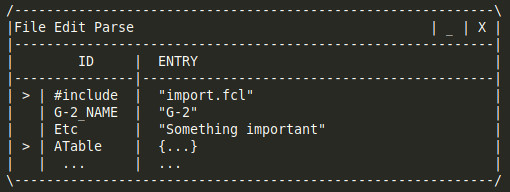
\includegraphics[width=10cm]{exampleLayout.jpg}
          \caption{A potential layout for a simple FHiCL editor}
          \label{exampleLayout}
        \end{center}
      \end{figure}

    
    The functionality would be that users could edit or create extra entries using this interface. If the user desires to edit the \#include or just view the file to be included, double clicking the entry row with the \#include statement would open a second window containing the contents of that file. Alternatively, it could expand in place inserting the entries after the statement.

    For this approach, it should be noted that a common notice given was that during coding most of the time a program is syntactically incorrect as most of the time programmers are editing lines of code which may not make sense. As such, It would be recommended to have ANTLR only parse the resulting FHiCL file after the user specifically calls it - hopefully after they complete any edits and to their eyes seems syntactially correct. Otherwise, it is possible that the continuous re-parsing of the document may introduce latency, creating a bad user experience. 

    NOTE: Generally, ANTLR does not like tree modification. However, there is an addChild() function in ParserRuleContext that can add subtrees.


\end{itemize}

\section{Data Structures Used}
	\subsection{ANTLR-Generated}
		\quad ATNLR employs a vector-based tree as the method of containing all parsed materials. The tree is to be traversed from left to right with a DFS like algorithm. The tree consists of two types of nodes: TerminalNode and ErrorNode. ErrorNodes are placed if the token does not fit the parser's rules and it is able to recover by single token deletion or looping tests. Otherwise, the rest of the tree is populated by TerminalNodes. In the tree all of the leaves are generated by lexer rules and will contain a string that the lexer found. Each node contains one token which can then be accessed for the information encoded in the token. Seeing as how in each node we can access anything encoded in the token, creating a custom token may be beneficial to hold additional information if Fermilab wishes to expand FHiCL functionality. The following figures (Figures ~\ref{fig:fullTree} thru ~\ref{fig:exampleTrees}) show example trees. In Figure ~\ref{fig:exampleTrees} the main data will be held in the regular boxes and additional tokens such as white space and ":" are also tokens, but can be ignored, those tokens are in grey. Note that we don't need to visit those nodes, and as such is a potential point for optimization. 

		\begin{figure}[htbp]
      \begin{center}
        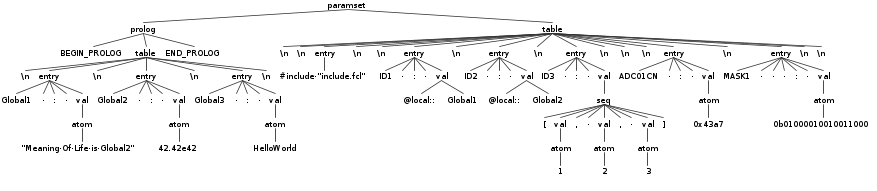
\includegraphics[width=13cm]{antlr4.png}
        \caption{ANTLR-generated parse tree of a simple FHiCL file}
        \label{fig:fullTree}
      \end{center}
    \end{figure}
		\begin{figure}[htbp]
      \begin{center}
        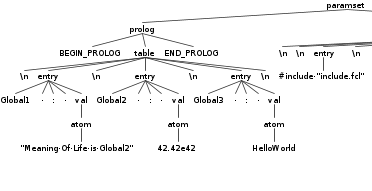
\includegraphics[width=13cm]{antlr4_section.png}
        \caption{ANTLR-generated parse tree close-up}
        \label{fig:justProlog}
      \end{center}
    \end{figure}
    \begin{figure}[!htbp]
      \begin{center}
        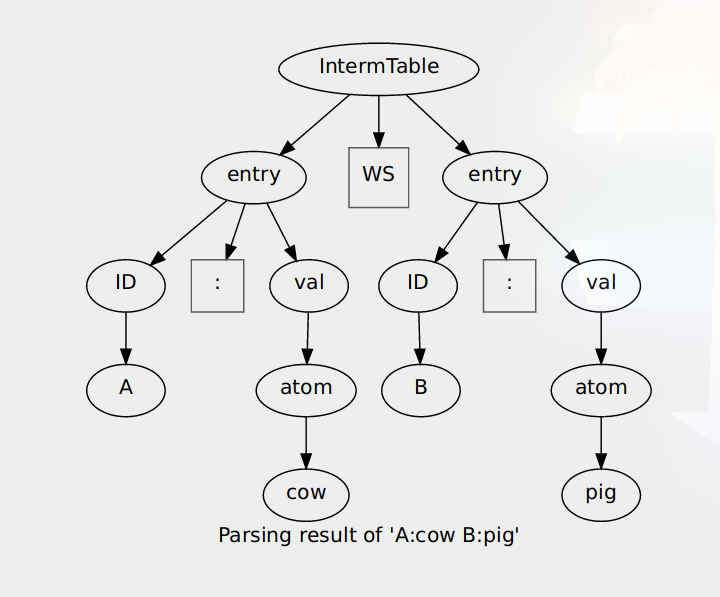
\includegraphics{regular.png}
        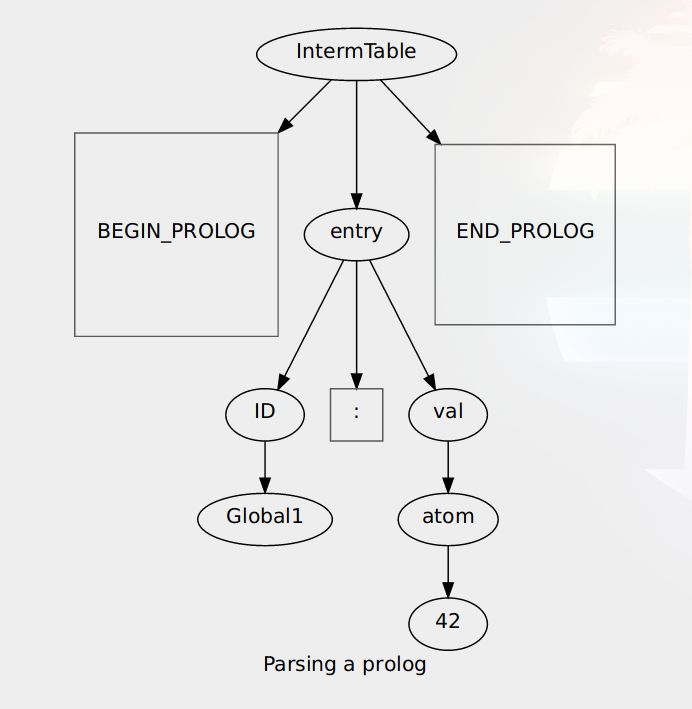
\includegraphics{prolog.png}
        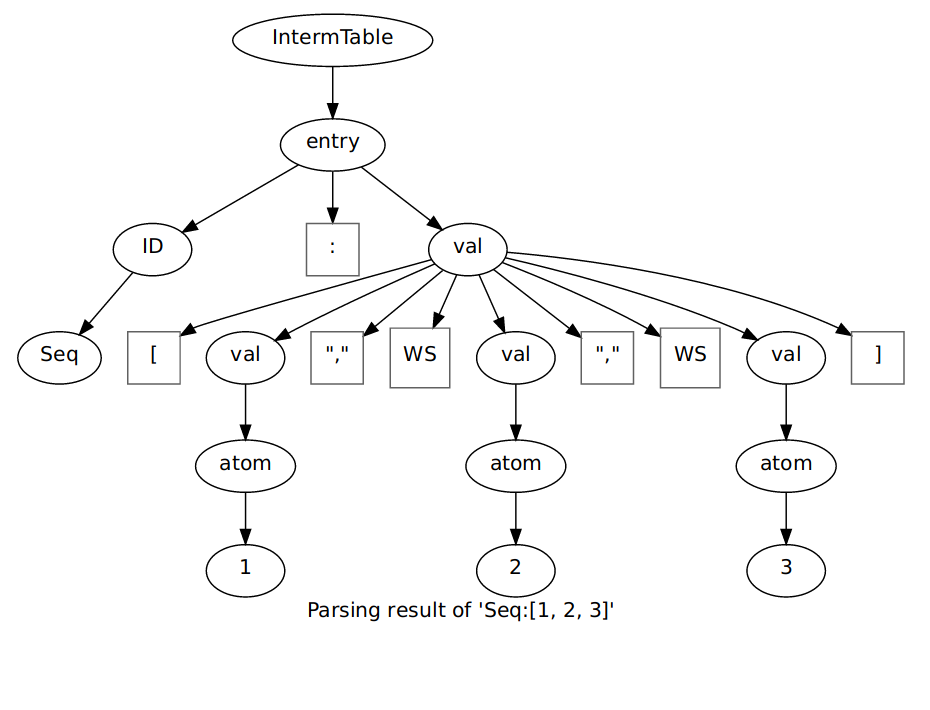
\includegraphics{Sequence.png}
        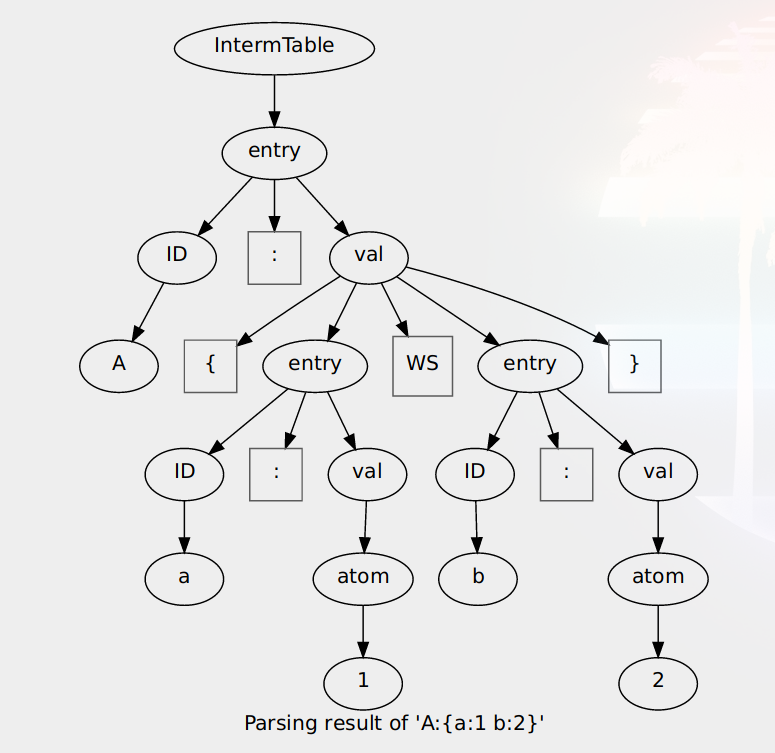
\includegraphics{Table.png}
        \caption{resulting parse trees from basic FHiCL constructs}
        \label{fig:exampleTrees}
      \end{center}
    \end{figure}
	

	\subsection{intermediate table/extendedval}
		\quad Currently, it seems that for the generation of a configuration from a FHiCL document the current implementation of the intermediate table and extendedval with slight modifications would be simplest way forward. It is easier to use the ANTLR generated tree for any debugging required, simplifying the actual data structure required for regular use. That being said, another alternative is to expand extendedval to hold all information that could be beneficial in the debugging process such as overwrite histories.

    Potential modifications to the current fhicl data structures could be implemented to allow easier integration with the ANTLR method of parsing. Extended\_value and ParameterSet currently hold everything required, however, they require re-writes to change from boost::any to std::any. The intermediate\_table implementation can be expanded to use ANTLR features to remove some functions in detail pertaining to determination of type.

\section{Potentially useful ANTLR things.}
\begin{itemize}
  \item Error Checking \\
      \quad Error nodes allow for ANTLR to populate a parse tree even if your config is syntactically incorrect. On top of that, ANTLR can catch these errors and return the line and position of the offense, as well as explain the error and what it was expecting. 

  \item Ease of Modification \\
      \quad The entirety of the ANTLR runtime's code is available, and modification is encouraged. If one desired, they could re-write the lexer and parser (easier on smaller languages). As such, ANTLR is incredibly customizable. Additionally, potential optimizations could be made by creating a custom token class (with corresponding token factory) to more easily send additional information to the parser or visitor. 

 \item Grammar Actions\\
      \quad The grammar can directly call functions while it is lexing or parsing. These are quite useful especially for more complex languages (which FHiCL may or may not fit depending on future expansion.) 

      Additionally, there are many tools in the lexer to assist with ambiguity resolution. 
\end{itemize}
\section{Conclusion}
	Overall, ANTLR is a promising and viable candidate to replace the current FHiCL parser. ANTLR has the funcitonality required for all actions required by FHiCL with additional tools that can be used to expand if the need arises. 
\end{document}